\documentclass[fleqn]{beamer}

\usepackage[british]{babel}
\usepackage{verbatim}
\usepackage{graphicx,hyperref,ru,url}

\title[Plaintext Recovery Attacks against SSH]{
Review: Plaintext Recovery Attacks against SSH}

\subtitle{Introduction to Cryptographic Algorithms '12/'13}

\author[Estourgie \& Br\"ucker]{
Raoul Estourgie\\
Ben Br\"ucker}

\institute[Radboud University Nijmegen]{
  Institute for Computing and Information Sciences \\
  Radboud University Nijmegen}

\date[Presentation 5-4-2013]

\begin{document}

  \begin{frame}
    \titlepage
  \end{frame}

  \begin{frame}
    \frametitle{Outline}
    \tableofcontents
  \end{frame}
  
\section{Introduction}

  \begin{frame}
    \frametitle{Introduction}
	\begin{block}{Test Block}
	Fancy Block
	\end{block}
	Other text
  \end{frame}

  \begin{frame}
    \frametitle{Test}
    \begin{center}
    \includegraphics[scale=1]{drawing.pdf}
    \end{center}
  \end{frame}
  
    \begin{frame}
    \frametitle{Test}
    \begin{center}
    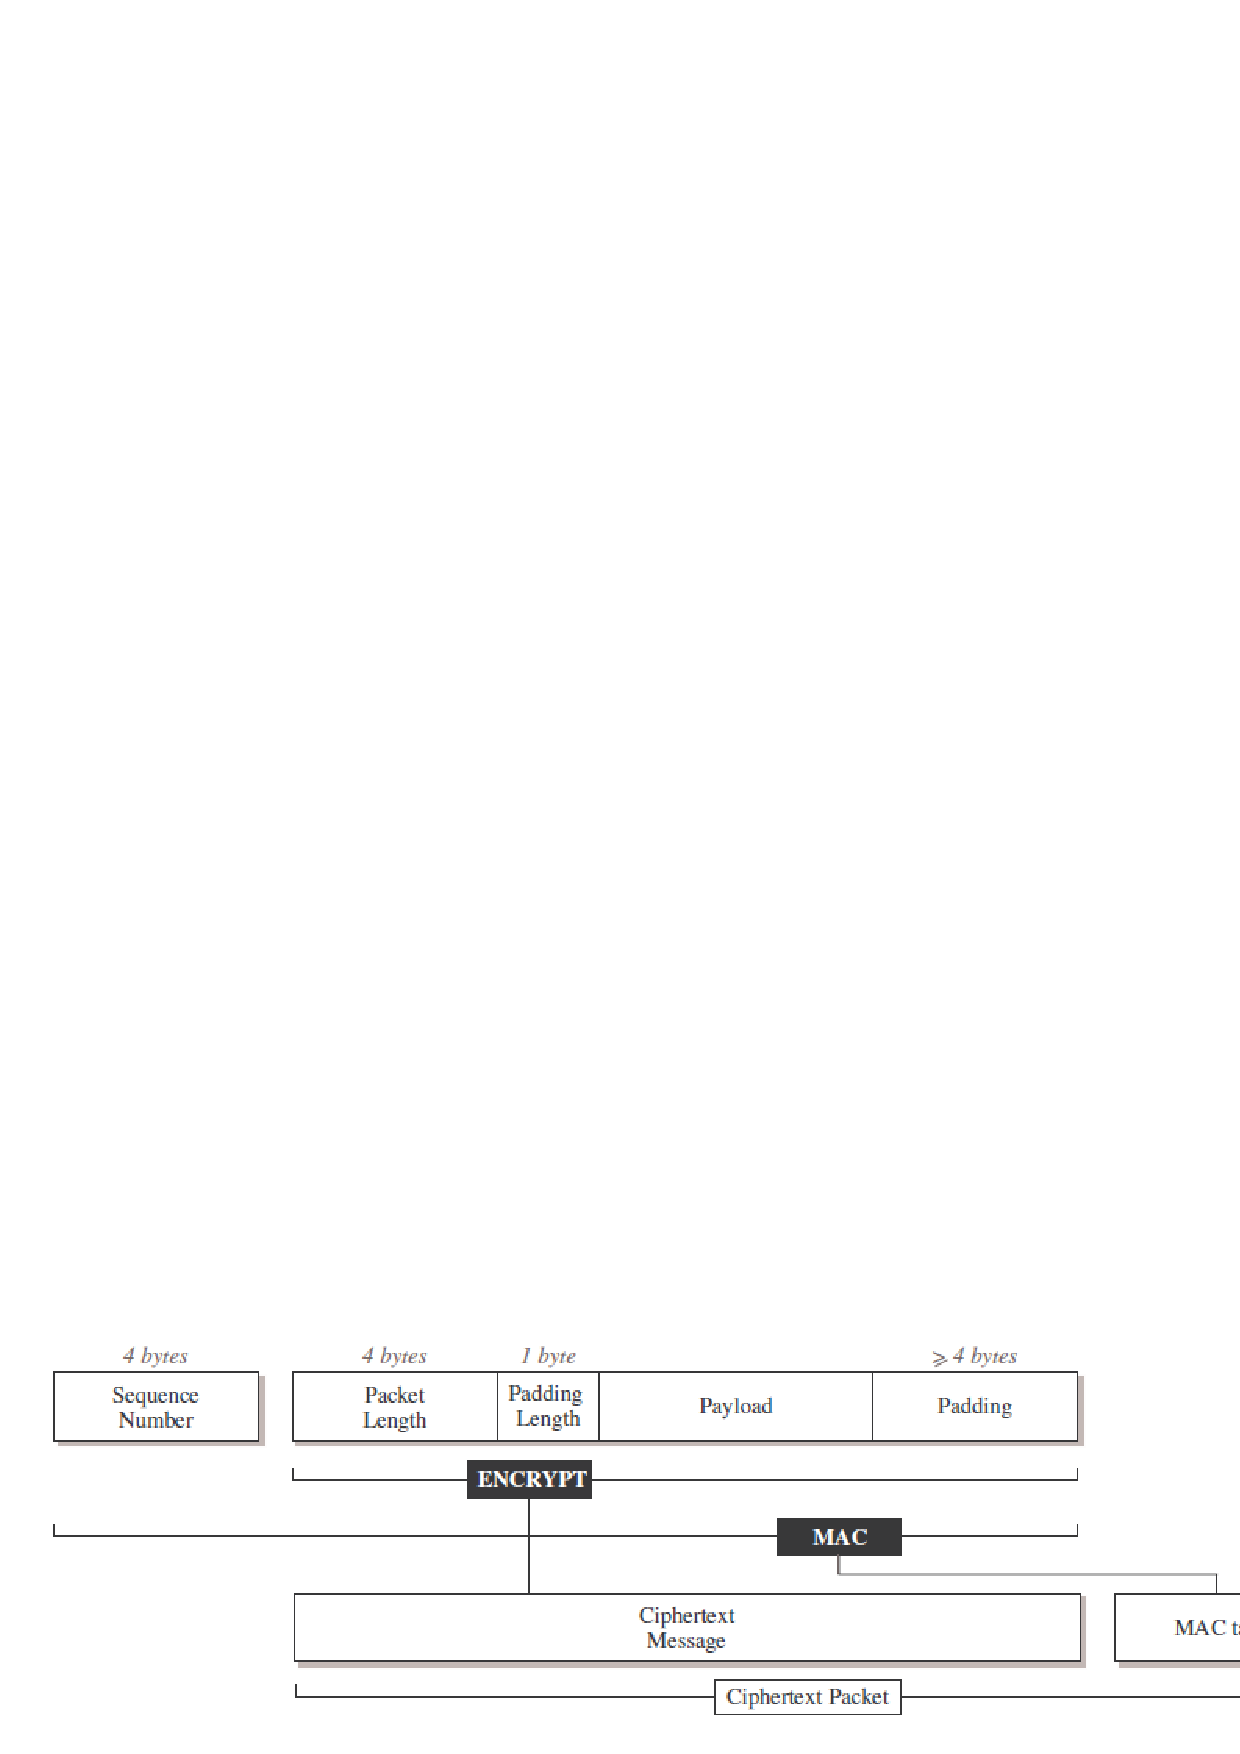
\includegraphics[scale=1]{SSHBPP.pdf}
    \end{center}
  \end{frame}
  
\section{Questions}

  \begin{frame}
    \frametitle{Questions}
    \begin{center}
    Questions?
    \end{center}
  \end{frame}
\end{document}
